\documentclass[journal=jacsat,manuscript=article]{achemso}

\usepackage{cmap}
\pdfgentounicode=1
\input glyphtounicode
\usepackage[utf8]{inputenc}
\usepackage[T1]{fontenc}

\SectionNumbersOn
\setkeys{acs}{maxauthors = 10, etalmode = truncate}

\usepackage[english]{babel}
\usepackage[version=3]{mhchem}
\usepackage{xr}
\usepackage{xcolor}
\usepackage{hyperref}

\frenchspacing
\externaldocument{supporting}



%%%%%%%%%%%%%%%%%%%%%%%%%%%%%%%%%%%%%%%%%%%%%%%%%%%%%%%%%%%%%%%%%%%%%

\newcommand\ex[1]{\ensuremath{^{\text{\scriptsize #1}}}}
\newcommand\e[1]{\ensuremath{_{\text{\scriptsize #1}}}}

\newcommand\todo[1]{\textcolor{red}{[#1]}}

%%%%%%%%%%%%%%%%%%%%%%%%%%%%%%%%%%%%%%%%%%%%%%%%%%%%%%%%%%%%%%%%%%%%%

\def\affIRCP{Chimie ParisTech, PSL University, CNRS, Institut de Recherche de Chimie Paris, 75005 Paris, France}

\author{Fran\c{c}ois-Xavier Coudert}
\affiliation{\affIRCP}
\email{fx.coudert@chimieparistech.psl.eu}

\title{Working title}


\begin{document}

\begin{tocentry}
Abstract will go here.
\end{tocentry}

\begin{abstract}
todo
\end{abstract}
\clearpage

%%%%%%%%%%%%%%%%%%%%%%%%%%%%%%%%%%%%%%%%%%%%%%%%%%%%%%%%%%%%%%%%%%%%%
\section{Introduction}

Lorem ipsum dolor sit amet, consectetur adipiscing elit. Phasellus urna eros, condimentum non commodo ac, condimentum in felis. Sed lectus felis, mattis sit amet rutrum et, imperdiet quis ex. Quisque ornare ante at diam fermentum tincidunt. In a augue nunc. Proin a dui vitae sapien venenatis ullamcorper. Nulla facilisi. In hac habitasse platea dictumst. Fusce quis nisl nec dolor ullamcorper facilisis et at arcu. Donec varius auctor nisl in consectetur.\cite{Zhao2025}

You can refer to figures in the main text or supporting info, as can be seen in \autoref{fig:workflow} and \autoref{fig:supp_workflow}. Tables work the same, see \autoref{tab:metrics} for details.

\begin{figure}[ht]
    \centering
    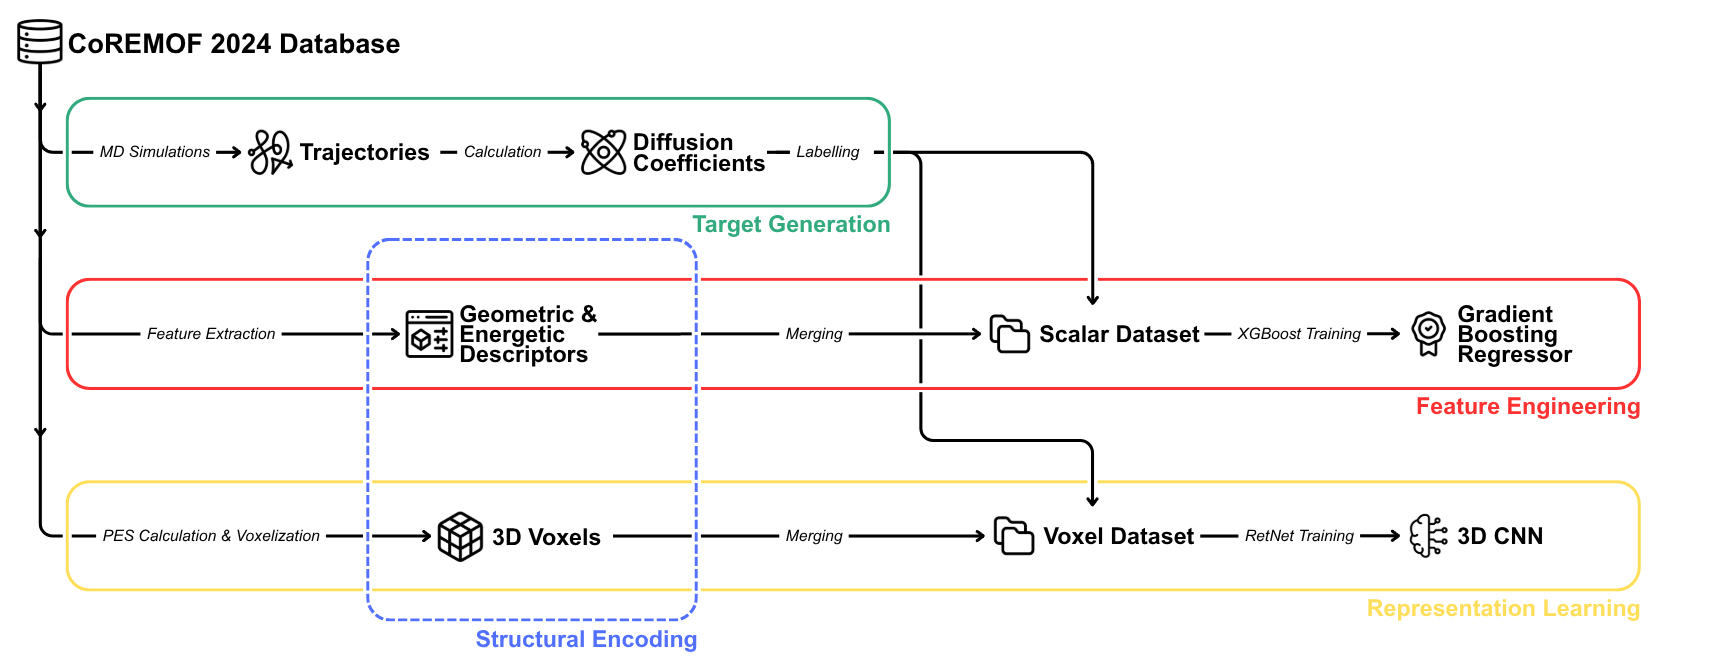
\includegraphics[width=0.8\linewidth]{figures/workflow.png}
    \caption{Schematic representation of the computational workflow.}
    \label{fig:workflow}
\end{figure}


\begin{table}[ht]
    \centering
    \caption{Predictive performance and computational efficiency of the evaluated models.}
    \begin{tabular}{llcccc}
    \hline
    Gas & Method & RMSE & MAE & $R^2$ & Training Time \\
    \hline
    Xe & Standard Method & --    & --    & --    & --   \\
    Xe & Voxelized PES   & 0.330 & 0.471 & 0.863 & 3h31 \\
    \hline
    Kr & Standard Method & --    & --    & --    & --   \\
    Kr & Voxelized PES   & 0.286 & 0.398 & 0.879 & 3h43 \\
    \hline
    Kr & Voxelized PES (MaxPool) & 0.244 & 0.347 & 0.911 & 3h33 \\
    \hline
    \end{tabular}
    \label{tab:metrics}
\end{table}


%%%%%%%%%%%%%%%%%%%%%%%%%%%%%%%%%%%%%%%%%%%%%%%%%%%%%%%%%%%%%%%%%%%%%
\section{Materials and Methods}



%%%%%%%%%%%%%%%%%%%%%%%%%%%%%%%%%%%%%%%%%%%%%%%%%%%%%%%%%%%%%%%%%%%%%

\section{Results and discussion}


\section{Conclusions \& Perspectives}


%%%%%%%%%%%%%%%%%%%%%%%%%%%%%%%%%%%%%%%%%%%%%%%%%%%%%%%%%%%%%%%%%%%%%

\begin{acknowledgement}
This work was funded by XXX. Access to high-performance computing platforms was provided by YYY. We thank ZZZ.
\end{acknowledgement}

\begin{suppinfo}
XXX, yyy, zzz.
\end{suppinfo}

\bibliography{article}

\end{document}